\section{System Designs}
In this section, all of the design aspects of this system have been detailed and justified. This includes the design of the user interface itself, the navigation and expected user path through the application, and the internal design of the application.

\subsection{User Interface Design}
In this section, the interface for each of the main pages of the application have been displayed, along with justifications for why they were designed the way they were. Before any work was completed on the project, designs for each of these pages were produced, and shared with the client. The finale designs were then based on his feedback, and the combination of the best features from all the designs produced. These initial designs can be found in {\color{red} appendix A} and are referenced throughout this section.
s
\paragraph{Route Discovery Page/Landing Page}\ \\
\begin{figure}[!ht]
	\vspace{-5mm}
	\begin{center}
		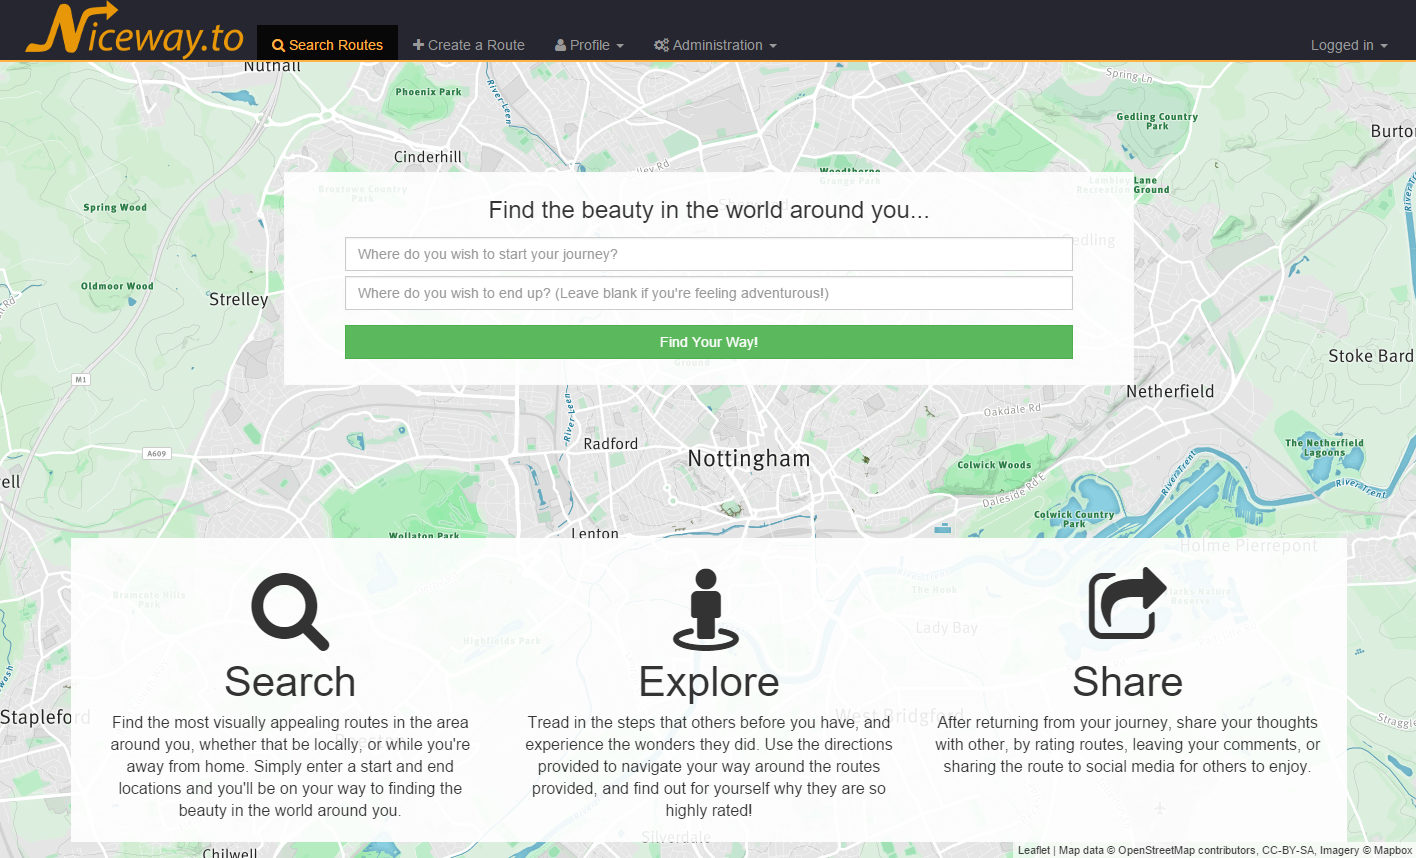
\includegraphics[width=0.8\textwidth]{images/design/landing.png}
	\end{center}
	\vspace{-5mm}
\end{figure}

{\color{red}
\noindent 
Why it is good\ \\
What was taken from each of the designs in the appendix\ \\
How it addresses the problem \ \\
Why it is designed the way it is\ \\
What differences there are to the designs
}

\paragraph{Route Listing Page}\ \\
\begin{figure}[!ht]
	\vspace{-5mm}
	\begin{center}
		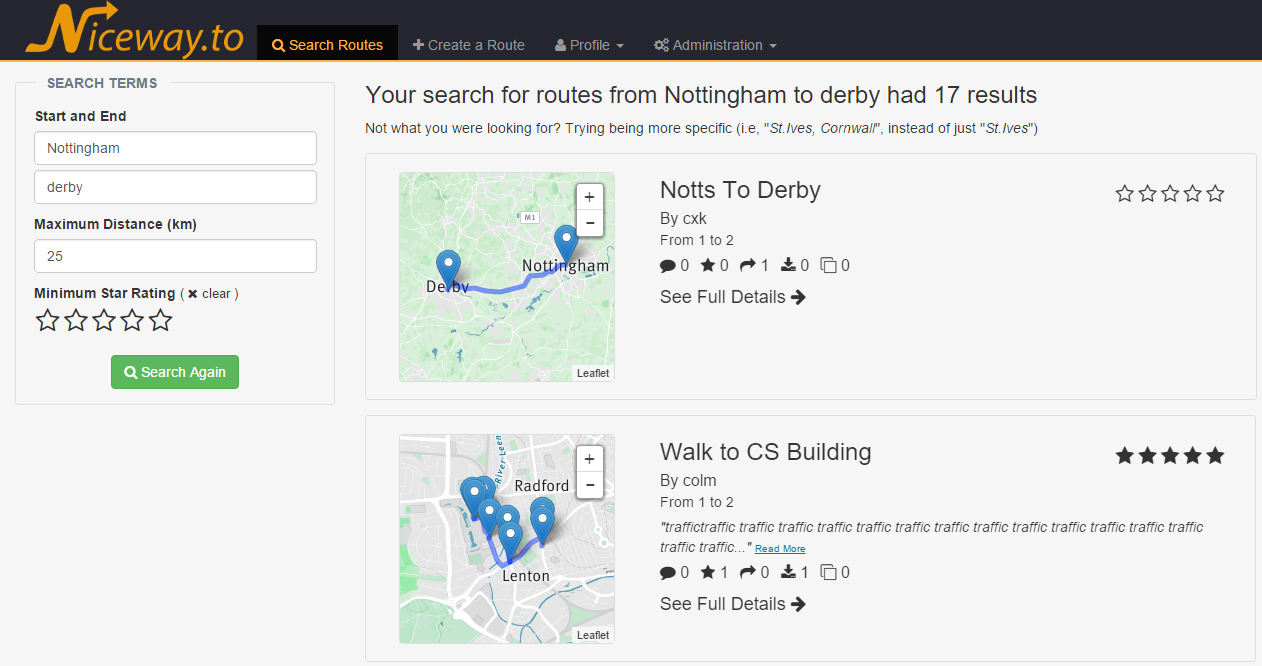
\includegraphics[width=0.5\textwidth]{images/design/listing.png}
	\end{center}
	\vspace{-10mm}
\end{figure}

{\color{red}
\noindent 
Why it is good\ \\
What was taken from each of the designs in the appendix\ \\
How it addresses the problem \ \\
Why it is designed the way it is\ \\
What differences there are to the designs
}

\newpage 
\paragraph{Route Detail Page}\ \\
\begin{figure}[!ht]
	\vspace{-5mm}
	\begin{center}
		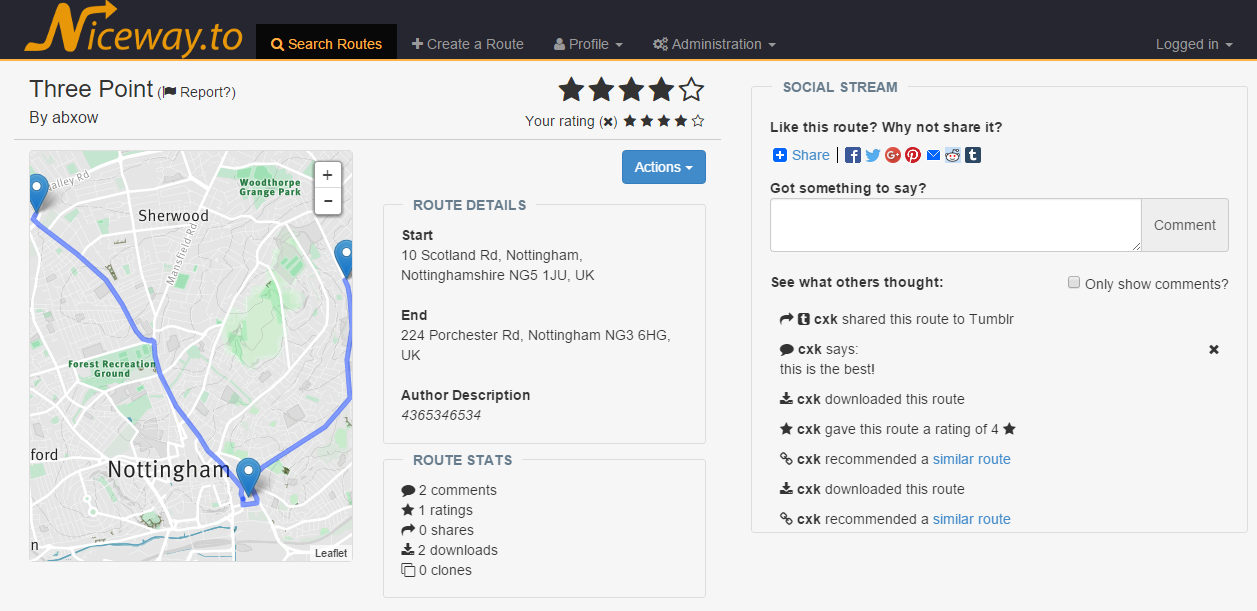
\includegraphics[width=0.7\textwidth]{images/design/detail.png}
	\end{center}
	\vspace{-5mm}
\end{figure}

{\color{red}
\noindent 
Why it is good\ \\
What was taken from each of the designs in the appendix\ \\
How it addresses the problem \ \\
Why it is designed the way it is\ \\
What differences there are to the designs
}

\paragraph{Route Creation Page}\ \\
\begin{figure}[!ht]
	\vspace{-5mm}
	\begin{center}
		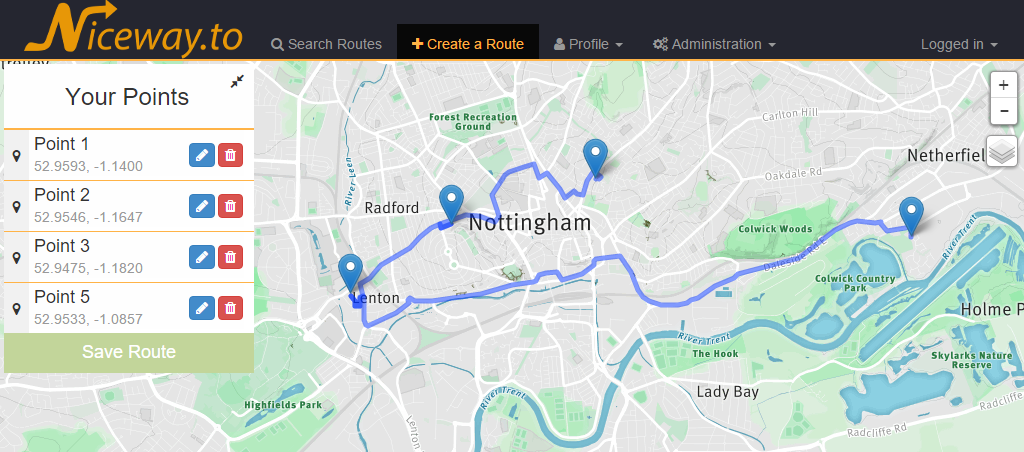
\includegraphics[width=0.7\textwidth]{images/design/create.png}
	\end{center}
	\vspace{-5mm}
\end{figure}

{\color{red}
\noindent 
Why it is good\ \\
What was taken from each of the designs in the appendix\ \\
How it addresses the problem \ \\
Why it is designed the way it is\ \\
What differences there are to the designs
}
{\color{blue} main client feedback was more social - so implemented the social stream to emphasize}

\paragraph{My Account Page}\ \\
\begin{figure}[!ht]
	\vspace{-5mm}
	\begin{center}
		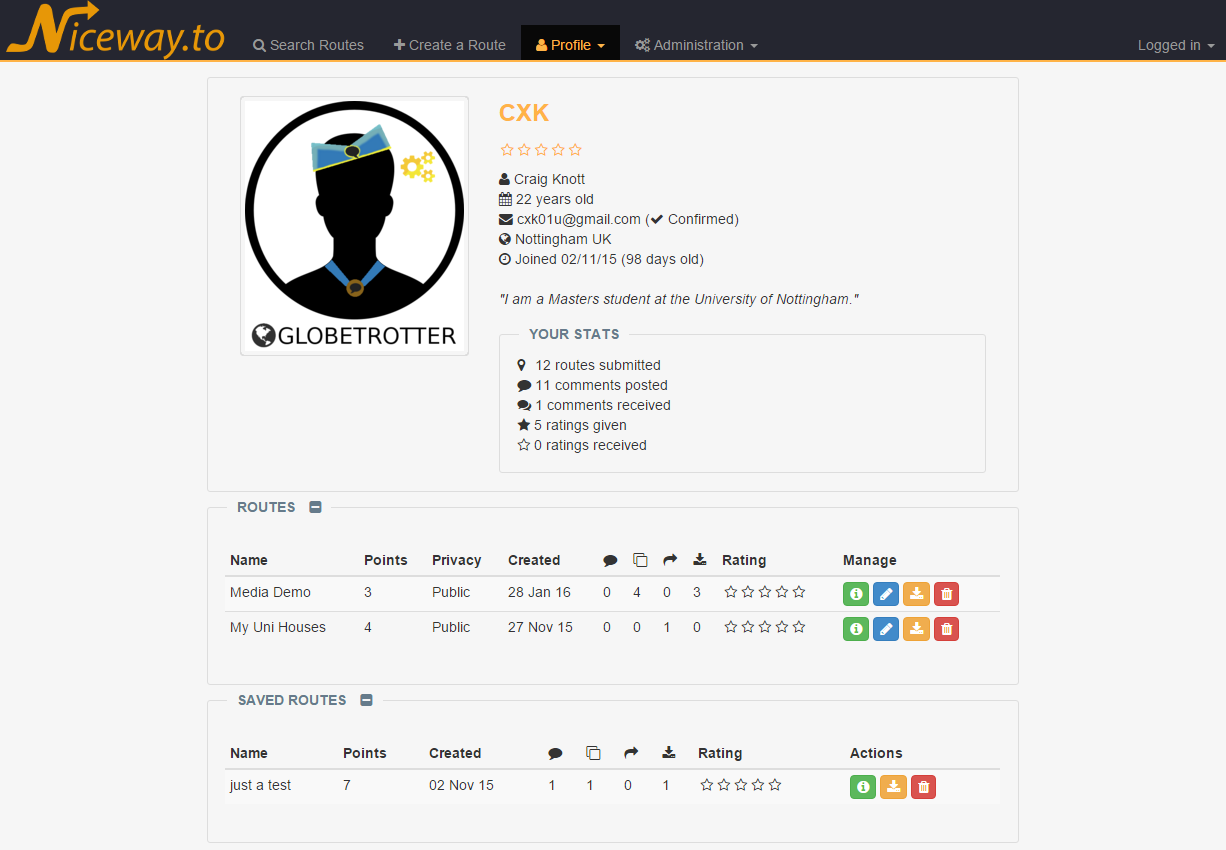
\includegraphics[width=0.5\textwidth]{images/design/profile.png}
	\end{center}
	\vspace{-5mm}
\end{figure}

{\color{red}
\noindent 
Why it is good\ \\
What was taken from each of the designs in the appendix\ \\
How it addresses the problem \ \\
Why it is designed the way it is\ \\
What differences there are to the designs
}
\ \\
\ \\
\noindent
{\color{red}
Mention the magic number seven / white space is not your enemy stuff
White Space is Not Your Enemy: \cite{golombisky2013white}\ \\
\ \\A
The magical number seven, plus or minus two: \cite{miller1956magical} - only put a certain number of things on the screen at once\ \\
\ \\
Could I have the menu please? An eye tracking study of design conventions \cite{mccarthy2004could} - how navigation and elements on the page generally start on the left because that's where people (in western culture at least) will look first\ \\
\ \\
Colour appeal in website design within and across cultures: A multi-method evaluation  \cite{cyr2010colour} - how colours have been used to group actions - green is pos, red is neg\ \\
\ \\
Interface design technique to simplify and declutter your interfaces \cite{depot2014clutter} - icons, placeholders, controls on demand, hovers and modals\ \\
\ \\
McDougall - uses are more likely to 'like' icons if they recognise them, which is why using well known icons was important, hence fontawesome/glyphicons \cite{mcdougall2008like}
}

\subsubsection{Heuristic Evaluation of the Interface}
In this section, the user interface is evaluated using several key metrics. These include the general purpose usability heuristics identified by Jakob Nielsen\cite{nielsen199510}, and the golden rules of interface design identified by Ben Schneiderman\cite{shneiderman2005designing}. The purpose of this section is to highlight how the interface conforms to these metrics, and why they are important within the context of the application.\ \\
\ \\
{\color{red}
	These have been grouped total, and the specific heuristics being referenced as in brackets, with the initials of the author, and the number of that heuristic. - these heuristics are listed in appendix D
	//in the format jakobs hueristics - JN1 - abc, JN2- def, ....
	 \ \\
	\ \\
Visibility and Feedback (JN1, BS3)\ \\
User should be in full control (JN3, JN7, BS4, BS7, BS8)\ \\
Consistency (JN4, BS1)\ \\
Error prevention and Recovery (JN5, JN9, BS5, BS6)\ \\
Cognitive Load (JN6, BS8)\ \\
Aesthetic and minimalist design (JN10)\ \\
Match between system and the real world (JN2)\ \\
}


\subsection{Navigation/Control Flow Design}

{\color{blue}



In the final design of the system, there were x main sections, which have been listed below:
\begin{enumerate}
	\item Route discovery - what it is
	\item Route listing  - what it is
	\item Route detail - what it is
	\item Route creation - what it is
	\item Profile page - what it is
	\item Admin page - what it is
	\item Login/Signup - what it is
\end{enumerate}
}

{\color{blue}
	when desigining the website, it's important to think about how users will travel through the site, depending on what their goals are. For niceway.to, there will be two main user groups: those with accounts (exports - activity and regularly contribute), and those without accounts (travellers, most using the search), whose paths would be different.
}
{\color{blue}	
the general path for non use,as shown in figure y is landing page, results, then detail page. This is why they are designed as they are: on search, they want to search, so box is very visible, like google, then results  - clearly laid out results with ability to re-search if mistakes, and then detail page, display everything about the route, but ability to look deeper if user so wishes\ \\
\ \\
the general path for the expert user would be different. generally would involve logging in and checking social interaction on their owns, and routes that they follow, as well as: general path for expert - login in, look at my account, check out new social interactions on their routes, look at friends routes, create a new route, update skins. diagram shows this. how does design facilitate this?
}

{\color{blue} 
	of course some users may not follow this path, and it is not the only bath. user has freedom to traverse to essentially any page at any point (excluding logged in only pages, and the search results to details page). important for promoting freedom and a sense of control within the system. The user is free to decide how they wish to travel through the system, and this means they are free to traverse forward or backward through the system to make any alterations, or fix any mistakes they may have made.
}

\subsection{Internal Design}
{\color{blue} 
	using a model view controller design pattern because of x, y, z advantages. figure 10 shows this interaction. when a page is requested, we hit the controller, this processes stuff, makes some db calls using the models (which abstract the db), then we pass the data to the view and display this. this means the view never talks directly to the data. to make pages interactive / updatable, we use ajax calls to request more data or specific actins (defined in the contorller). at this point, it was decided to use php with the zend framework (reasons for which are described in section \ref{sec:kid})which helps to enforce this model\ \\
	\ \\
	diagram of db, model, controller, view, ajax, client and server, base controller subclasses and modelfactory subclass
}


